\chapter{Evaluation} \label{chapter:evaluation}
This chapter evaluates the malicious capabilities developed in our rootkit by comparing them to the original objectives we presented at the beginning of our research in section \ref{section:project_objectives}. For this, we will analyse whether our rootkit meets the expected functionality by simulating a machine infection in a virtualized environment. A rootkit functionality will be considered fulfilled in the case it can be reproduced successfully in the experimental environment.

As we mentioned, the following are the functionalities we seeked to implement in our rootkit:
\begin{itemize}
\item Hijacking the execution of user programs while they are running, injecting libraries and executing malicious code, without impacting their normal execution.
\item Featuring a command-and-control module powered by a network backdoor, which can be operated from a remote client. This backdoor should be controlled with stealth in mind, featuring similar mechanisms to those present in rootkits found in the wild.
\item Tampering with user data at system calls, resulting in running malware-like programs and for other malicious purposes.
\item Achieving stealth, hiding rootkit-related files from the user.
\item Achieving rootkit persistence, the rootkit should run after a complete system reboot.
\end{itemize}

\section{Experimental setting}
The test environment that will be used to showcase the rootkit functionalities consists on two virtual machines running under Oracle VM VirtualBox \cite{virtualbox_page}. One of them will be the host infected with the rootkit, while the other will be used as the attacker machine from which to operate the rootkit client. 

Both virtual machines will be connected via a bridged adapter, as figure \ref{fig:vm_setting_bridged} shows. With this virtual networking setting, the virtual machines connect to a device driver of the host system which injects the data received from the physical network \cite{bridged_networking}. From the virtual machine point of view, both the attacker and the infected machine appear to be physically connected (via a network cable) to the same network interface, each with a different assigned IP address. The name of this interface will be "enp0s3".

\begin{figure}[htbp]
	\centering
	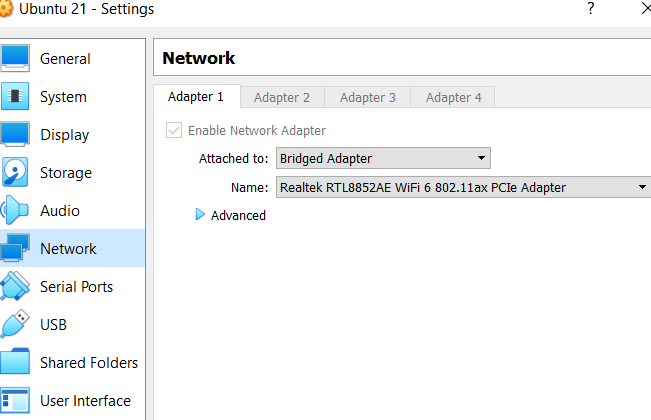
\includegraphics[width=13cm]{vm_setting_bridged.png}
	\caption{Network settings for both of the VMs on the test environment.}
	\label{fig:vm_setting_bridged}
\end{figure}

Table \ref{table:vm_config_test_environment} shows the role and charactersitics of the two machines. The overall test environment configuration with the described settings is illustrated in figure \ref{fig:test_env}.

\begin{table}[H]
\begin{tabular}{|>{\centering\arraybackslash}p{3cm}|>{\centering\arraybackslash}p{3cm}|}
\hline
\multicolumn{2}{|c|}{\textbf{INFECTED MACHINE}}\\
\hline
\textbf{Attribute} & \textbf{Value}\\
\hline
\hline
User & osboxes\\
\hline
Operating System & GNU/Linux\\
\hline
Distribution & Ubuntu 21.04\\
\hline
Kernel version & 5.11.0-49\\
\hline
IP address & 192.168.1.124\\
\hline
\end{tabular}
\quad
\begin{tabular}{|>{\centering\arraybackslash}p{3cm}|>{\centering\arraybackslash}p{3cm}|}
\hline
\multicolumn{2}{|c|}{\textbf{ATTACKER MACHINE}}\\
\hline
\textbf{Attribute} & \textbf{Value}\\
\hline
\hline
User & RED\\
\hline
Operating System & GNU/Linux\\
\hline
Distribution & Ubuntu 18.04\\
\hline
Kernel version & 5.4.0-96\\
\hline
IP address & 192.168.1.121\\
\hline
\end{tabular}
\caption{Configuration of virtual machines in the test environment.}
\label{table:vm_config_test_environment}
\end{table}

\begin{figure}[htbp]
	\centering
	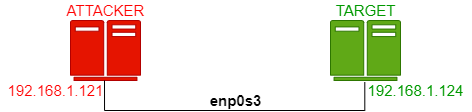
\includegraphics[width=13cm]{test_env.png}
	\caption{Network topology of test environment.}
	\label{fig:test_env}
\end{figure}


%Maybe this is not the place for story telling? I thought that telling it like this fits nicely here to put some context, but I can try to change it.
\section{Attack scenario} \label{section:attack_scenario}
This section presents an hypothetical attack scenario, covering each of the steps the attacker must follow in order to prepare the rootkit and infect a machine:

A security researcher called 'RED' has managed to exploit a high-severity RCE vulnerability in a critical system controlled by an adversary which was found exposed to the Internet (e.g.: not behind a NAT \cite{nat_comptia}). After this exploitation, RED has now spawned a reverse shell connection with the privileged user 'osboxes', but he knows that the system is often rebooted and that he may lose access soon. Furthermore, the vulnerability he exploited is already well-known and may get patched in the near future, so he needs to persist his access. RED decides to load a classic rootkit consisting of a malicious kernel module, but he finds out that this capability is restricted in the system (e.g.: kernel.modules\_disabled=1 \cite{kernel_modules_restrict}), so he must find an alternative approach. At some point, RED realises that even if kernel modules were restricted, the system administrator did not block eBPF, so he decides to use TripleCross.

Firstly, RED creates a secret directory where to hide the rootkit, and downloads it, as shown in figure \ref{fig:post_exp}.

\begin{figure}[htbp]
	\centering
	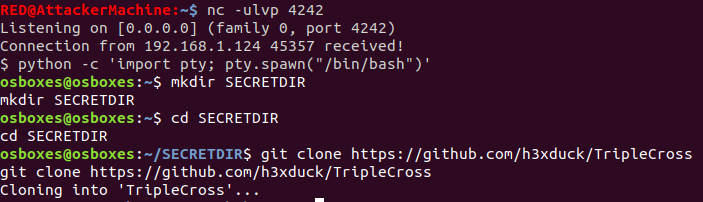
\includegraphics[width=13cm]{sch_post_exp.png}
	\caption{Creation of hidden directory and downloading rootkit.}
	\label{fig:post_exp}
\end{figure}

The rootkit C2 capabilities work out of the box, but RED wants to use all of the rootkit modules, so he must first make some configurations. Table \ref{table:rootkit_config} shows the configurations and the files to modify for each module.

\begin{table}[htbp]
\begin{tabular}{|>{\centering\arraybackslash}p{2cm}|>{\centering\arraybackslash}p{3cm}|>{\centering\arraybackslash}p{4cm}|>{\centering\arraybackslash}p{4cm}|}
\hline
\textbf{MODULE} & \textbf{FILENAME} & \textbf{CONSTANT} & \textbf{DESCRIPTION}\\
\hline
\hline
Execution hijacking & src/common/ constants.h & PATH\_EXECUTION\_HIJACK\_PROGRAM & Absolute path of malicious program\\
\hline
Privilege escalation & src/common/ constants.h & STRING\_FS\_SUDOERS\_ENTRY & Entry to inject in sudoers file\\
\hline
Library injection & src/helpers/ injection\_lib.h & ATTACKER\_IP \& ATTACKER\_PORT & IP address and port of attacker machine\\
\hline
Persistence module & src/helpers/ deployer.sh & CRON\_PERSIST \& SUDO\_PERSIST & Values to store at persistence files\\
\hline
\end{tabular}
\caption{Overall rootkit modules configuration.}
\label{table:rootkit_config}
\end{table}

Once the appropiate values have been written, RED executes the \textit{packager.sh} script, that will compile the rootkit. Alternatively, an attacker could have compiled it locally and sent it to the remote machine afterwards.

After the script execution finishes, a folder \textit{apps} is generated with all the rootkit files. This directory contains all the files and scripts needed for the rootkit installation. RED now executes the \textit{deployer.sh} script, which installs the rootkit and writes the persistence files, as shown in figure \ref{fig:deploy_root}

\begin{figure}[htbp]
	\centering
	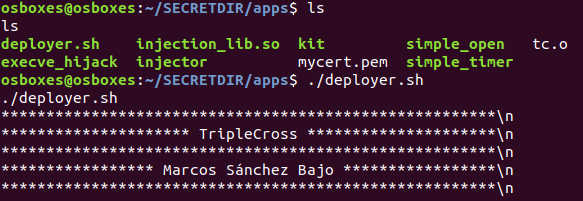
\includegraphics[width=13cm]{sch_deploy_root.png}
	\caption{Files created by packager.sh and execution of deployer.sh.}
	\label{fig:deploy_root}
\end{figure}

Once the script has been executed, all rootkit modules are loaded and the backdoor is already waiting for commands. RED can now close the reverse shell and open the rootkit client. He now has persistent privileged access to the infected machine.

\section{Hijacking execution of running processes}
Following the infection process described in section \ref{section:attack_scenario}, TripleCross can hijack the execution of running processes by means of the library injection module. This module incorporates two sample programs (\textit{src/helpers/simple\_timer.c and src/helpers/simple\_open.c}), both containing the execution of one of the hijacked syscalls (sys\_timerfd\_settime and sys\_openat respectively). Additionally, the functionality can be tested in any process of the infected machine by changing its settings. Table \ref{table:lib_injection_config} shows how to customize the functionality of the library injection module.

\begin{table}[htbp]
\begin{tabular}{|>{\centering\arraybackslash}p{3cm}|>{\centering\arraybackslash}p{5.5cm}|>{\centering\arraybackslash}p{5.5cm}|}
\hline
\textbf{FILENAME} & \textbf{CONSTANT} & \textbf{DESCRIPTION}\\
\hline
\hline
src/common/ constants.h & TASK\_COMM\_NAME\_INJECTION\_TARGET\_TIMERFD\_SETTIME & Name of process to hijack at syscall sys\_timerfd\_settime.\\
\hline
src/common/ constants.h & TASK\_COMM\_NAME\_INJECTION\_TARGET\_OPEN & Name of process to hijack at syscall sys\_openat.\\
\hline
src/helpers/ injection\_lib.c & ATTACKER\_IP \& ATTACKER\_PORT & IP address and port of attacker machine\\
\hline
\end{tabular}
\caption{Library injection module configuration.}
\label{table:lib_injection_config}
\end{table}

After a successful injection the malicious library will run a reverse shell against the attacker machine. Also, it will print a message for us to check it locally. Therefore, from the attacker machine, we will listen to the specified IP and port, considering the injection successful if a connection is opened.


\subsection{Test program simple\_timer}
Table \ref{table:lib_injection_config_simple_timer} shows the module configuration for running this attack.

\begin{table}[htbp]
\begin{tabular}{|>{\centering\arraybackslash}p{3cm}|>{\centering\arraybackslash}p{5.5cm}|>{\centering\arraybackslash}p{5.5cm}|}
\hline
\textbf{FILENAME} & \textbf{CONSTANT} & \textbf{VALUE}\\
\hline
\hline
src/common/ constants.h & TASK\_COMM\_NAME\_INJECTION\_TARGET\_TIMERFD\_SETTIME & "simple\_timer"\\
\hline
src/helpers/ injection\_lib.c & ATTACKER\_IP \& ATTACKER\_PORT & 192.168.1.127 \& 5555 \\
\hline
\end{tabular}
\caption{Library injection module configuration for attacking simple\_timer.c.}
\label{table:lib_injection_config_simple_timer}
\end{table}

Figure \ref{fig:sc_lib_inj_simple_timer_off} shows the execution of the simple\_timer process without the rootkit installed.

\begin{figure}[htbp]
	\centering
	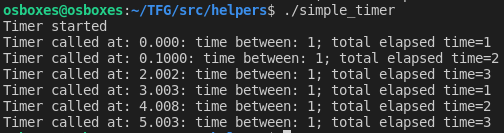
\includegraphics[width=13cm]{sch_sc_lib_inj_simple_timer_off.png}
	\caption{Normal execution of simple\_timer program.}
	\label{fig:sc_lib_inj_simple_timer_off}
\end{figure}

Once the rootkit is installed it starts the module automatically, looking for system calls from the simple\_timer process.
The attacker must in the mean time start a listener (e.g.: with netcat), as shown in figure \ref{fig:sc_lib_inj_nc}.

\begin{figure}[htbp]
	\centering
	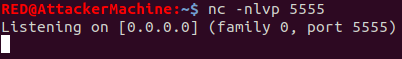
\includegraphics[width=12cm]{sch_sc_lib_inj_nc.png}
	\caption{Attacker waiting for a connection with netcat.}
	\label{fig:sc_lib_inj_nc}
\end{figure}

Then, the simple\_timer program gets executed on the infected machine. As we can observe in figure \ref{fig:sc_lib_inj_simple_timer_exec}, the injection suceeds and a message is printed from the library. 

\begin{figure}[htbp]
	\centering
	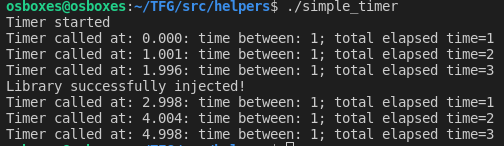
\includegraphics[width=12cm]{sch_sc_lib_inj_simple_timer_exec.png}
	\caption{Execution of simple\_timer.c with rootkit active.}
	\label{fig:sc_lib_inj_simple_timer_exec}
\end{figure}


Figure \ref{fig:sc_lib_inj_nc_success} shows the attacker connected to the reverse shell launched from the library.

\begin{figure}[htbp]
	\centering
	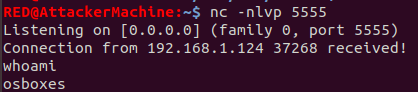
\includegraphics[width=12cm]{sch_sc_lib_inj_nc_success.png}
	\caption{Reverse shell received after library injection attack.}
	\label{fig:sc_lib_inj_nc_success}
\end{figure}


\subsection{Test program simple\_open}
The library injection module can also be tested with the simple\_timer program, which opens multiple files with sys\_openat. The rootkit configuration for this is shown in table \ref{table:lib_injection_config_simple_open}.

\begin{table}[htbp]
\begin{tabular}{|>{\centering\arraybackslash}p{3cm}|>{\centering\arraybackslash}p{5.5cm}|>{\centering\arraybackslash}p{5.5cm}|}
\hline
\textbf{FILENAME} & \textbf{CONSTANT} & \textbf{VALUE}\\
\hline
\hline
src/common/ constants.h & TASK\_COMM\_NAME\_INJECTION\_TARGET\_OPEN & "simple\_open"\\
\hline
src/helpers/ injection\_lib.c & ATTACKER\_IP \& ATTACKER\_PORT & 192.168.1.127 \& 5555 \\
\hline
\end{tabular}
\caption{Library injection module configuration for attacking simple\_open.c.}
\label{table:lib_injection_config_simple_open}
\end{table}

As we can observe in figure \ref{fig:sc_lib_inj_simple_open}, when the injection suceeds, a message is printed on screen. Also, the attacker receives a shell, like we showed in figure \ref{fig:sc_lib_inj_nc_success}.

\begin{figure}[htbp]
	\centering
	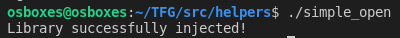
\includegraphics[width=12cm]{sch_sc_lib_inj_simple_open.png}
	\caption{Execution of simple\_open with rootkit active.}
	\label{fig:sc_lib_inj_simple_open}
\end{figure}


\subsection{Hijacking systemd}
Apart from the test programs, the library injection module can also inject the malicious library on any process of the system that makes use of either sys\_openat or sys\_timerfd\_settime. By hijacking privileged system programs such as systemd, the malicious library can achieve automatic root permissions once it is run (although these are anyways automatically granted via the privilege escalation module). Table \ref{table:lib_injection_config_systemd} shows the module configuration for running an attack against this process.

\begin{table}[htbp]
\begin{tabular}{|>{\centering\arraybackslash}p{3cm}|>{\centering\arraybackslash}p{5.5cm}|>{\centering\arraybackslash}p{5.5cm}|}
\hline
\textbf{FILENAME} & \textbf{CONSTANT} & \textbf{VALUE}\\
\hline
\hline
src/common/ constants.h & TASK\_COMM\_NAME\_INJECTION\_TARGET\_TIMERFD\_SETTIME & "systemd"\\
\hline
src/common/ constants.h & TASK\_COMM\_NAME\_INJECTION\_TARGET\_OPEN & "systemd"\\
\hline
src/helpers/ injection\_lib.c & ATTACKER\_IP \& ATTACKER\_PORT & 192.168.1.127 \& 5555 \\
\hline
\end{tabular}
\caption{Library injection module configuration for attacking the systemd process.}
\label{table:lib_injection_config_systemd}
\end{table}

With these configurations, we can run the rootkit and wait for systemd to call one of these syscalls. Eventually this call occurs, and using the debug messages of the rootkit we can get information on what happened, as shown in figure \ref{fig:sch_sc_lib_inj_systemd_debug}.

\begin{figure}[htbp]
	\centering
	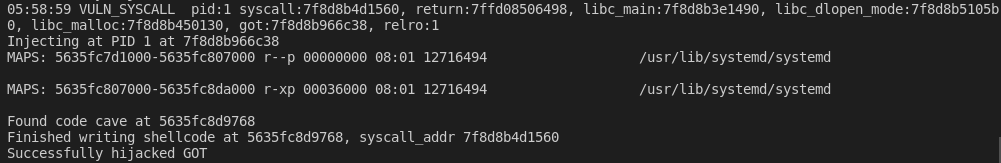
\includegraphics[width=12cm]{sch_sc_lib_inj_systemd_debug.png}
	\caption{Rootkit debug messages showing library injection.}
	\label{fig:sc_lib_inj_systemd_debug}
\end{figure}

As we can observe in the figure, the rootkit finds the relevant addresses via the technique we described on section \ref{section:lib_injection} and proceeds to overwrite the GOT address. The library is loaded and executed, and since systemd is executed by the root user, the attacker receives a root shell as shown in figure \ref{fig:lib_inj_success_root}. Most importantly, the systemd process does not crash after this attack.

\begin{figure}[htbp]
	\centering
	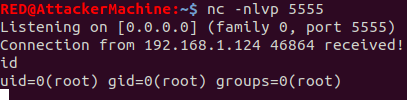
\includegraphics[width=12cm]{sch_lib_inj_success_root.png}
	\caption{Reverse shell received with root user after systemd library injection.}
	\label{fig:lib_inj_success_root}
\end{figure}


\section{Backdoor and C2}
The backdoor module works out of the box without any additional configurations needed. It includes the C2 capabilities and the rootkit client used to communicate with the backdoor. As we described in section \ref{subsection:rootkit_manual}, the client allows for the operations listed on table \ref{table:rootkit_client_actions}.

\begin{table}[htbp]
\begin{tabular}{|>{\centering\arraybackslash}p{5cm}|>{\centering\arraybackslash}p{9.5cm}|}
\hline
\textbf{PROGRAM ARGUMENTS} & \textbf{ACTION DESCRIPTION}\\
\hline
\hline
./injector -c <Victim IP> & Spawns a plaintext pseudo-shell by using the execution hijacking module.\\
\hline
./injector -e <Victim IP> & Spawns an encrypted pseudo-shell by commanding the backdoor with a pattern-based trigger.\\
\hline
./injector -s <Victim IP> & Spawns an encrypted pseudo-shell by commanding the backdoor with a multi-packet trigger (of both types).\\
\hline
./injector -p <Victim IP> & Spawns a phantom shell by commanding the backdoor with a pattern-based trigger.\\
\hline
./injector -a <Victim IP> & Orders the rootkit to activate all eBPF programs.\\
\hline
./injector -a <Victim IP> & Orders the rootkit to detach all of its eBPF programs.\\
\hline
./injector -S <Victim IP> & Showcases how the backdoor can hide a message from the kernel.\\
\hline
./injector -h & Displays help.\\
\hline
\end{tabular}
\caption{Rootkit client options.}
\label{table:rootkit_client_actions}
\end{table}

Once the rootkit is installed, the backdoor is launched automatically and will wait for backdoor triggers ready to launch the corresponding requested actions.

\subsection{Spawning encrypted pseudo-shells}
Encrypted pseudo-shells can be spawned using the rootkit client either with pattern-based or multi-packet backdoor triggers.

\textbf{Pattern-based triggers}\\
When using a pattern-based trigger, the attacker must indicate the following information:
\begin{itemize}
\item The IP address of the infected machine.
\item The network interface to use for sending the trigger.
\end{itemize}

As figure \ref{fig:sc_eps_rc} shows, the backdoor executes the requested action and starts an encrypted pseudo-shell connection with privileged permissions in which the attacker can introduce commands to be executed. Whenever the connection shall be closed, the attacker introduces the "EXIT" global command (as we explained in section \ref{subsection:rootkit_manual}), which ends the transmission gracefully.

\begin{figure}[htbp]
	\centering
	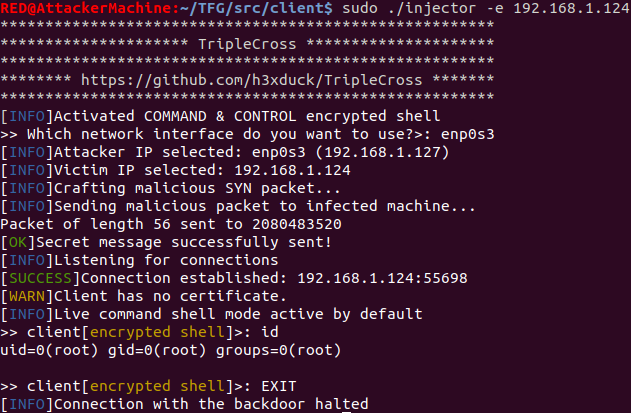
\includegraphics[width=12cm]{sch_sc_eps_rc.png}
	\caption{Encrypted pseudo-shell with rootkit client using pattern-based trigger.}
	\label{fig:sc_eps_rc}
\end{figure}

\textbf{Multi-packet triggers}\\
The rootkit client offers multiple options when using the multi-packet backdoor triggers. In particular, the attacker must specify the following fields:
\begin{itemize}
\item The IP address of the infected machine.
\item The network interface to use for sending the trigger.
\item Whether to hide the payload at the TCP sequence numbers or at the TCP source port.
\end{itemize}

Figure \ref{fig:sc_eps_seqnum} shows how the rootkit client asks for this data and spawns an encrypted pseudo-shell with the client when hiding the payload at the TCP sequence number. As we can observe in the figure, the payload is divided in 3 different chunks and injected to a stream of packets, which are sent in an orderly manner.

\begin{figure}[htbp]
	\centering
	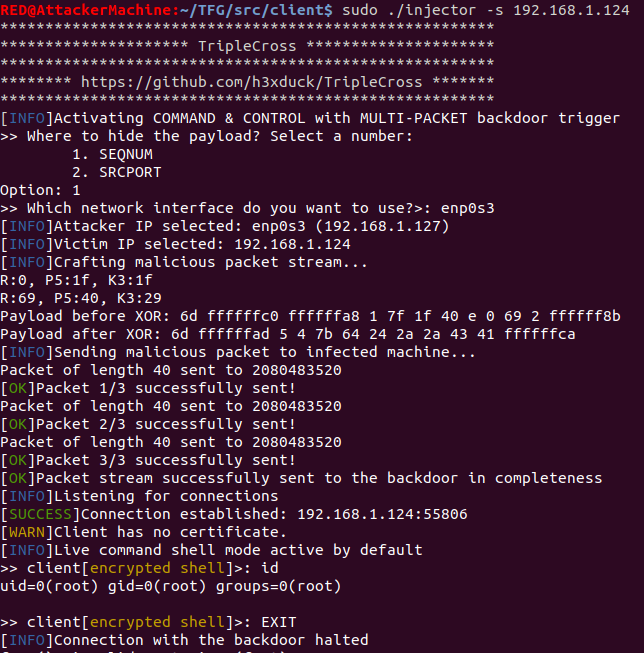
\includegraphics[width=12cm]{sch_sc_eps_seqnum.png}
	\caption{Encrypted pseudo-shell with rootkit client using multi-packet trigger with payload hidden in TCP sequence number.}
	\label{fig:sc_eps_seqnum}
\end{figure}

Figure \ref{fig:sc_eps_srcport} shows the same process but using the TCP source port as a means for hiding the data payload. As we can observe in the figure, in this case the paylaod is divided in 6 chunks.

\begin{figure}[htbp]
	\centering
	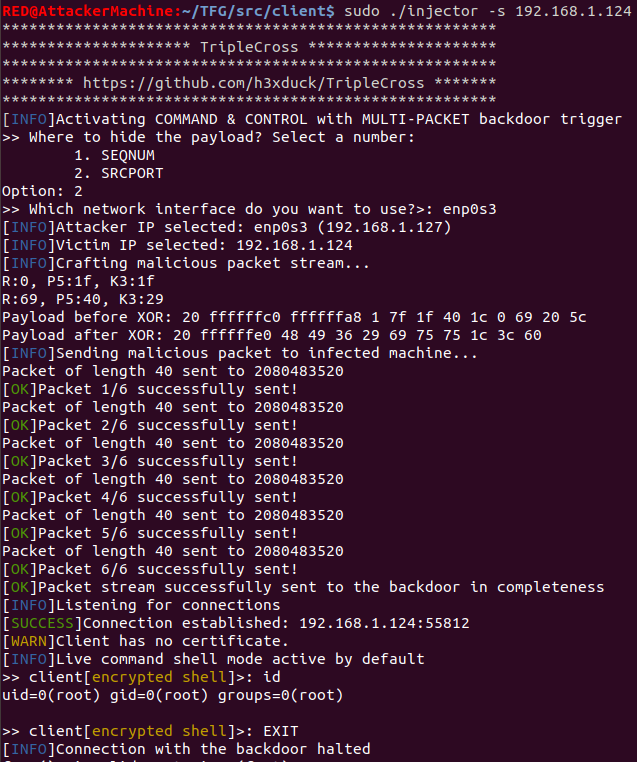
\includegraphics[width=12cm]{sch_sc_eps_srcport.png}
	\caption{Encrypted pseudo-shell with rootkit client using multi-packet trigger with payload hidden in TCP source port.}
	\label{fig:sc_eps_srcport}
\end{figure}

\subsection{Spawning phantom shells}




